\documentclass[11pt]{article}
\usepackage[margin=0.8in]{geometry}                % See geometry.pdf to learn the layout options. There are lots.
\geometry{letterpaper}                   % ... or a4paper or a5paper or ... 
%\geometry{landscape}                % Activate for for rotated page geometry
%\usepackage[parfill]{parskip}    % Activate to begin paragraphs with an empty line rather than an indent

\usepackage[colorlinks=true]{hyperref}
\usepackage{caption}
\usepackage{url}
\usepackage{biblatex}
\bibliography{bib/references}
\usepackage{subcaption}
\usepackage{graphicx}
\usepackage[section]{placeins}
\usepackage{amssymb}
\usepackage{epstopdf}

\DeclareGraphicsRule{.tif}{png}{.png}{`convert #1 `dirname #1`/`basename #1 .tif`.png}

\title{CSC 573 Project 2 : Simple FTP Service}
\author{Saurabh V. Pendse (ID: 001026185), Ashish J. Sharma (ID: 001043115)}
\date{\today}
%\date{}                                           % Activate to display a given date or no date

\begin{document}
\maketitle

All the experiments described in this document were performed on two physical hosts on the university private network. \textbf{The hosts were separate by $2$ hops}, as is evident from the output of the \verb|traceroute| command shown below : 

\begin{verbatim}
svpendse1@SVPNotebook:~$ traceroute 10.136.6.169

traceroute to vpna-01705.vpn.ncsu.edu (74.125.227.147), 64 hops max, 52 byte packets

 1  dc1-vpn-1.ncstate.net (152.1.18.4)  *  19 ms  *
 2  vpna-01705.vpn.ncsu.edu (10.136.6.169)  6 ms  7 ms  5 ms

svpendse1@SVPNotebook:~$ 
\end{verbatim}

Based on this setup, the retransmission timeout period (RTO) for the Go Back N as well as the Selective Repeat was set to $50$ milliseconds. This is following the TCP standard, where the RTO \textit{is set to twice} the Round Trip Time (RTT). The RTT in our case is approximately $25$ milliseconds (from the \verb|traceroute| command shown above). We now present the results obtained for each of the three tasks, first using the Go Back N strategy, followed by the Selective Repeat Strategy.

\section{Go Back N Strategy}
	\label{sec:gbn}
	\subsection{Task 1 : Effect of Window Size $N$}	
	\label{subsec:task1gbn}
	\begin{figure}[h]
		\centering
		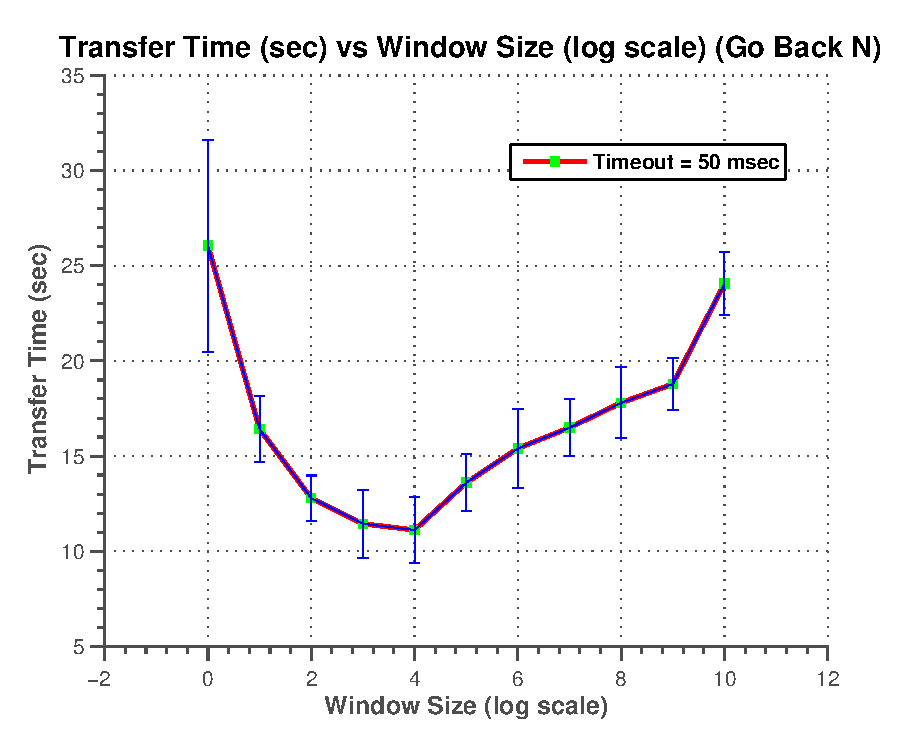
\includegraphics[width=0.5\linewidth]{../task1/figure_task1_gobackn.eps}
		\caption{Transfer Time (sec) vs Window Size (N) (log scale) using the Go Back N Strategy.}
		\label{fig:task1gbn}
	\end{figure}
		The parameters used for this experiment were as follows : 
		\begin{itemize}
			\item Loss Probability = $0.05$.
			\item File Size = $1$ MB.
			\item Maximum Segment Size (MSS) = $500$ bytes
		\end{itemize}	
		
		The Window Size ($N$) was varied from $1$ to $1024$ in the powers of $2$ (that is $1, 2, 4, 8, 16$ and so on). Each simulation was carried out 5 times and then averaged. The Figure \ref{fig:task1gbn} shows the time taken to transfer the file to the receiver when the window size at the host is varied. The X- axis is a logarithmic scale with the base $2$, e.g., a value of $2$ on the x-axis means a window size of $4$ ($2^{2}=4$).
		
		Theoretically, when using Go-Back-N with a small window size, a lot of time would be wasted in retransmitting the packets due to timeouts. A very large window size wouldn�t be optimal either as it can introduce error-recovery problems~\nocite{hall1999}. Error-recovery problem using Go-Back-N is the transmission of the same frames multiple times � if a frame or an ACK for that frame is lost, all frames following the frame that was lost are retransmitted~\nocite{tanenbaum2002}. This causes unnecessary delay in transmission. Thus, we need to find an optimum window size that would give us the minimum transmission time. That window size would exist between the two extreme conditions mentioned earlier.
		
This can be seen in the result of the simulation above.  On varying the window size from $1$ to $1024$ in powers of $2$, the minimum transmission time was achieved with the window size $16$ ($2^{4} = 16$) as seen from the graph. This is in agreement with the theoretical assumption we made above.

	\subsection{Task 2 : Effect of Segment Size MSS}
	\label{subsec:task2gbn}
	\begin{figure}[h]
		\begin{subfigure}[b]{0.49\linewidth}
			\centering
			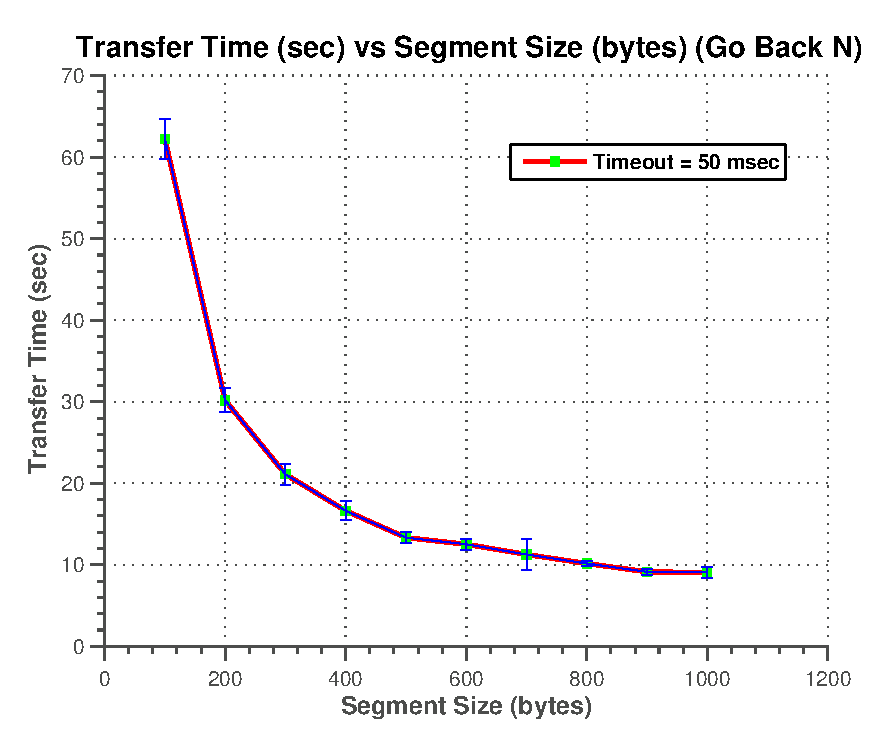
\includegraphics[width=\linewidth]{../task2/figure_task2_gobackn.eps}
			\caption{Transfer Time (sec) vs Maximum Segment Size (MSS) using the Go Back N Strategy.}
			\label{fig:task2gbn}
		\end{subfigure}
		\begin{subfigure}[b]{0.51\linewidth}
			\centering
			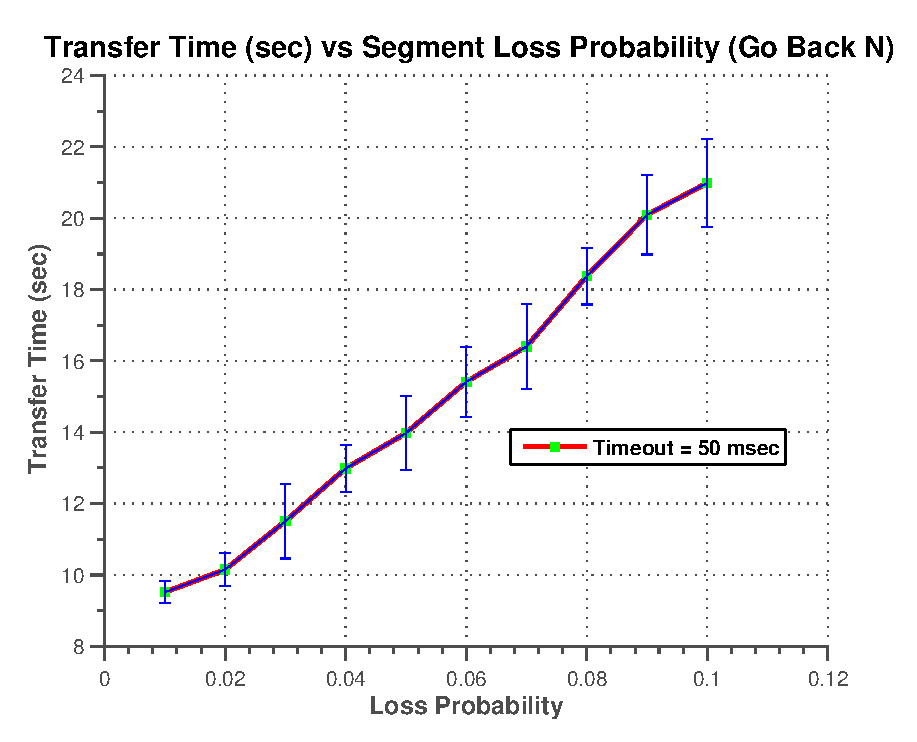
\includegraphics[width=\linewidth]{../task3/figure_task3_gobackn.eps}
			\caption{Transfer Time (sec) vs Loss Probability ($p$) using the Go Back N Strategy.}
			\label{fig:task3gbn}
		\end{subfigure}
	\end{figure}
	The parameters used for this experiment were as follows : 
		\begin{itemize}
			\item Loss Probability = $0.05$.
			\item File Size = $1$ MB.
			\item Window Size $N$ = 64.
		\end{itemize}		
		
		
		The MSS for the simulations was varied from 100 to 1000 bytes in increments of 100 bytes (that is, 100, 200, 300 and so on). Each simulation was carried out 5 times and then averaged.  The Figure \ref{fig:task2gbn} shows the variation of time taken to transfer the file to the receiver vs. the Maximum Segment Size. The X- axis in this graph has a linear scale.	
		
		The variation of the transfer time with respect to the segment size is related to the Bandwidth of the network rather than the flow control technique that is being used (Go-Back-N or Selective-Repeat). For example, for the same given bandwidth of the network, transmitting a file in 10 small segments would take a longer amount of time than transmitting it in 5 segments of larger size (assuming that the bandwidth-delay product is greater than the size of each segment). In other words, a smaller segment size in a network with high bandwidth doesn�t allow efficient utilization of the bandwidth and hence the transfer time is higher for a small MSS. As the MSS increases, the transfer time decreases. This theoretical assumption can be justified with the simulation results shown in the graph above.
However, the transfer time is not just a function of the segment size. It is also affected by the flow control technique (Go-Back-N in this case) being used. Go-Back-N uses a lot of time in re-transmissions due to lost or damaged ACKs - if a frame or an ACK for that frame is lost, all frames following the frame that was lost are retransmitted. Thus, we will see later in this report that even though the nature of the graph remains same when we use Selective-repeat, the transfer time decreases by a significant amount.

	\subsection{Task 3 : Effect of Loss Probability $p$}
	\label{subsec:task3gbn}
	The parameters used for this experiment were as follows : 
		\begin{itemize}
			\item Loss Probability : varied from $0.01$ to $0.1$ in increments of $0.01$.
			\item File Size = $1$ MB.
			\item Window Size $N$ = 64.
		\end{itemize}	
	
	The Figure \ref{fig:task3gbn} shows the variation of time taken to transfer the file to the receiver vs. the segment loss probability. The X- axis in this graph has a linear scale. 
	
	By logical reasoning, we can state that as the loss probability increases, the number of segments lost during transmission increases and hence the transmission time increases. This can be seen from the graph above where as the loss probability increases from 0.01 to 0.1, the transmission time increases from approximately 9 seconds to 21 seconds. 
	
As stated earlier, the transmission time is not just the function of the loss probability or the maximum segment size. Hence, when Selective Repeat is used for the same scenario instead of Go-Back-N, the nature of the graph remains same but the overall transmission time reduces significantly.  This has been elaborated in the Section \ref{subsec:task3selrepeat} of this document.
\newpage
\section{Selective Repeat Strategy}
	\label{sec:selrepeat}
	\subsection{Task 1}
	\label{subsec:task1selrepeat}
	\begin{figure}[h]
		\centering
		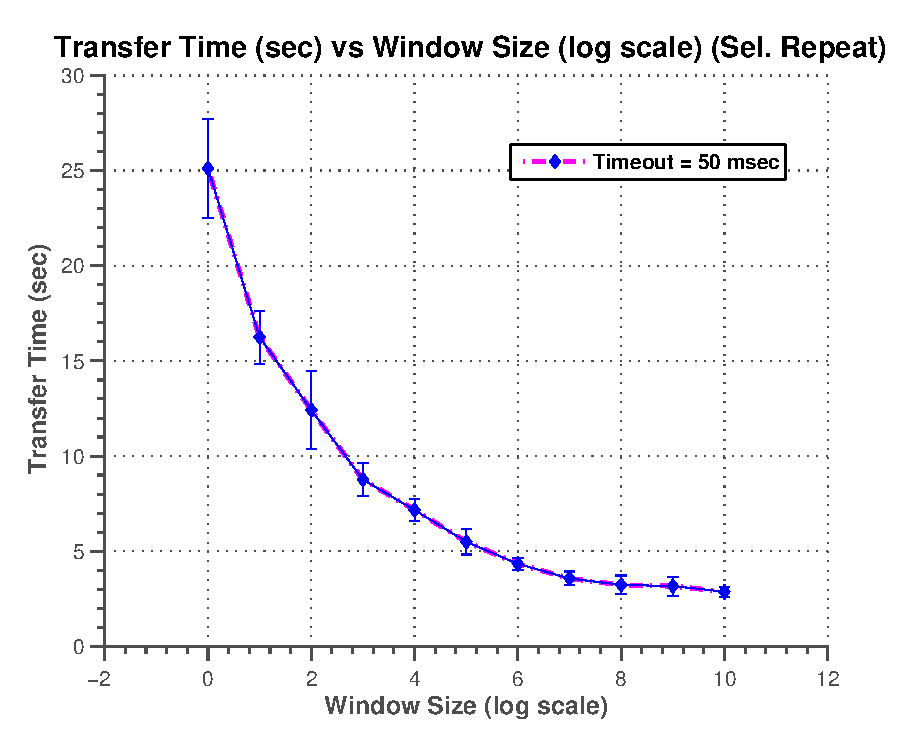
\includegraphics[width=0.5\linewidth]{../task1/figure_task1_selrepeat.eps}
		\caption{Average Transfer Time (sec) vs Window Size (N) (log scale) using the Selective Repeat Strategy.}
		\label{fig:task1selrepeat}
	\end{figure}
		The parameters used for this experiment were as follows : 
		\begin{itemize}
			\item Loss Probability = $0.05$.
			\item File Size = $1$ MB.
			\item Maximum Segment Size (MSS) = $500$ bytes
		\end{itemize}	
		
		The Window Size ($N$) was varied from $1$ to $1024$ in the powers of $2$ (that is $1, 2, 4, 8, 16$ and so on). Each simulation was carried out 5 times and then averaged. The Figure \ref{fig:task1selrepeat} shows the time taken to transfer the file to the receiver when the window size at the host is varied. The X- axis is a logarithmic scale with the base $2$, e.g., a value of $2$ on the x-axis means a window size of $4$ ($2^{2}=4$).
		
	The main difference between Selective-Repeat and Go-Back-N is that Go-Back-N uses cumulative ACK whereas Selective-Repeat sends ACK for each frame it receives~\nocite{tanenbaum2002}.  For example, if frames 1, 2, 3 and 4 were sent and frame 3 was lost, a receiver using Go-Back-N would send a cumulative ACK for frames up to frame 2. This means even if frame 4 was received, the sender would send it again as it has received cumulative ACK for frames only up to frame 2. However, if for the same scenario, a receiver uses the Selective-Repeat technique, it would send individual ACKs for frame 1, 2 and 4 and would store frame 4 in its buffer until frame 3 is retransmitted by the sender. When the sender does not receive an ACK for frame 3, it sends frame 3 again.
 
	The effect of the missing multiple transmissions of the same frame when using Selective-Repeat is evident from the graph above. As with Go-Back-N, when window size is small, the timeouts cause retransmissions and hence the transfer time is greater. However, as the window size increases, unlike Go-Back-N, the transmission time decreases as Selective-Repeat does not support cumulative ACKs and hence there are no duplicate transmissions. These theoretical assumptions have been justified by the simulation results plotted in the graph shown above.

	\subsection{Task 2}
	\label{subsec:task2selrepeat}
	\begin{figure}[h]
		\begin{subfigure}[b]{0.49\linewidth}
		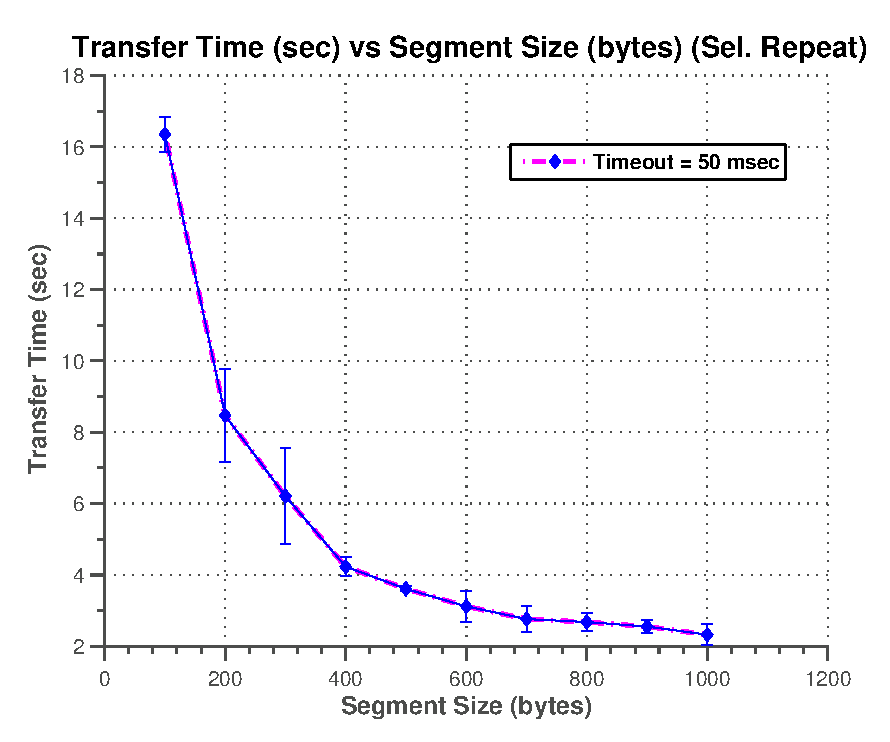
\includegraphics[width=\linewidth]{../task2/figure_task2_selrepeat.eps}
		\caption{Average Transfer Time (sec) vs Maximum Segment Size (MSS) using the Selective Repeat Strategy.}
		\label{fig:task2selrepeat}
		\end{subfigure}
		\begin{subfigure}[b]{0.51\linewidth}
		\centering
		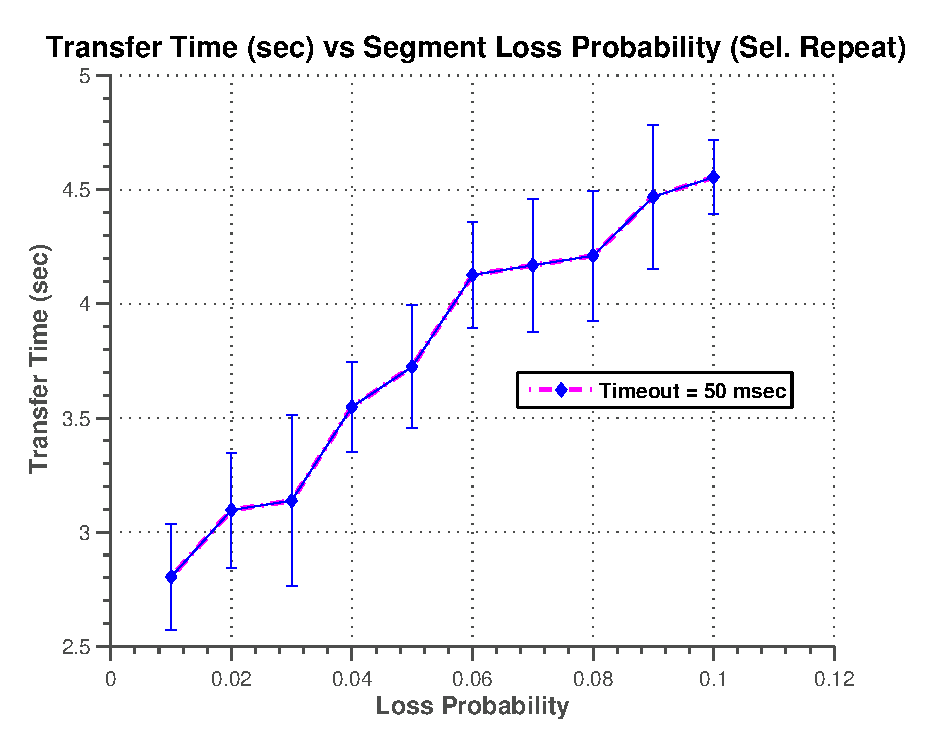
\includegraphics[width=\linewidth]{../task3/figure_task3_selrepeat.eps}
		\caption{Average Transfer Time (sec) vs Loss Probability ($p$) using the Selective Repeat Strategy.}
		\label{fig:task3selrepeat}
		\end{subfigure}
	\end{figure}
	
	The parameters used for this experiment were as follows : 
		\begin{itemize}
			\item Loss Probability = $0.05$.
			\item File Size = $1$ MB.
			\item Window Size $N$ = 64.
		\end{itemize}		
				
		The MSS for the simulations was varied from 100 to 1000 bytes in increments of 100 bytes (that is, 100, 200, 300 and so on). Each simulation was carried out 5 times and then averaged.  The Figure \ref{fig:task2selrepeat} shows the variation of time taken to transfer the file to the receiver vs. the Maximum Segment Size. The X- axis in this graph has a linear scale.	
		
		As discussed earlier, the nature of the graph is similar to what we saw with Go-Back-N. This is because the variation of the transfer time with respect to the segment size is primarily the property of the bandwidth of the network. 
		
		However, using the Selective-Repeat technique, the overall transmission time decreases when compared to Go-Back-N. This can be seen on the Y-axis. The reason behind this is the individual frame ACKs used by Selective-Repeat which eliminate the duplicate transmissions and thus improve the transmission time.
	
	\subsection{Task 3}	
	\label{subsec:task3selrepeat}
	
	The parameters used for this experiment were as follows : 
		\begin{itemize}
			\item Loss Probability : varied from $0.01$ to $0.1$ in increments of $0.01$.
			\item File Size = $1$ MB.
			\item Window Size $N$ = 64.
		\end{itemize}	
	
	The Figure \ref{fig:task3selrepeat} shows the variation of time taken to transfer the file to the receiver vs. the segment loss probability. The X- axis in this graph has a linear scale. 
	
	Theoretically, increase in loss probability would increase the loss and hence increase the transmission time. Thus, in the graph above, the nature remains the same as in case of Go-Back-N technique, but the overall transmission time reduces. The reason for the reduction of the transmission time is the absence of cumulative ACKs in Selective-Repeat as has been stated in the previous sections.

%\clearpage
\section{Comparison}
	
\begin{figure}[h]
        \begin{subfigure}[b]{0.48\linewidth}
                \centering
                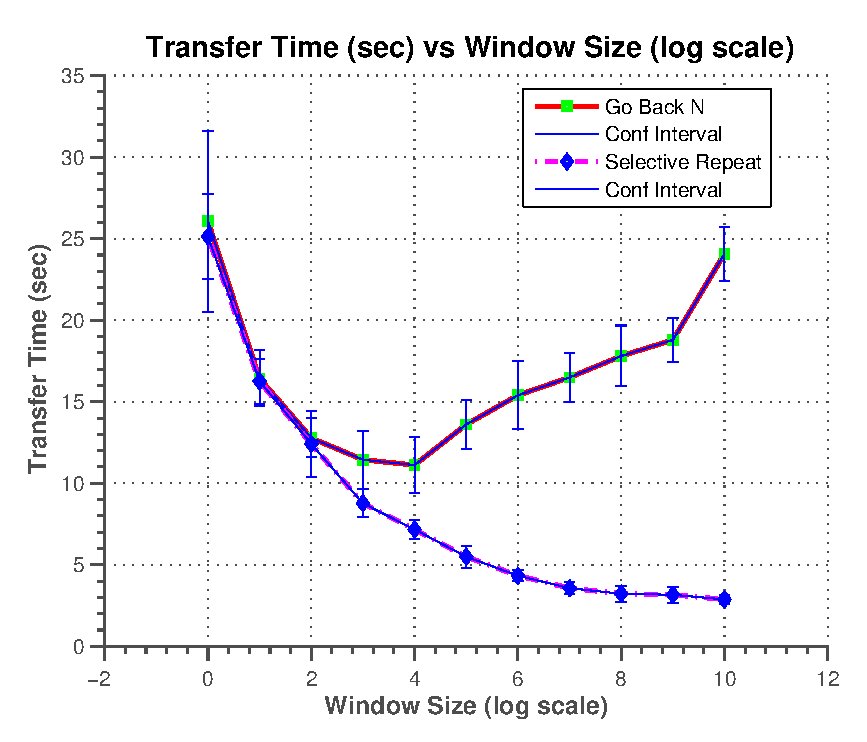
\includegraphics[width=\linewidth]{../task1/figure_task1_combined.eps}
                \caption{Average Transfer Time (sec) vs Window Size (N) for Go Back N and Selective Repeat Strategies.}
                \label{fig:task1combined}
        \end{subfigure}
        \begin{subfigure}[b]{0.48\linewidth}
                \centering
                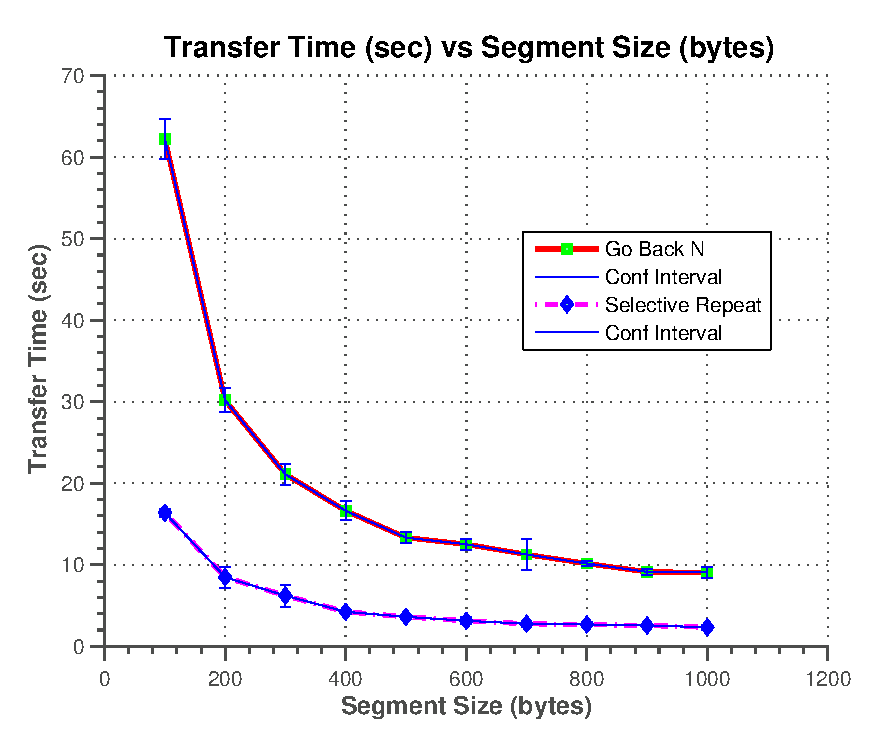
\includegraphics[width=\linewidth]{../task2/figure_task2_combined.eps}
                \caption{Average Transfer Time (sec) vs Maximum Segment Size (MSS) for Go Back N and Selective Repeat Strategies.}
                \label{fig:task2combined}
        \end{subfigure}
        \vspace{25pt}
        \begin{subfigure}[b]{0.48\linewidth}
                \centering
                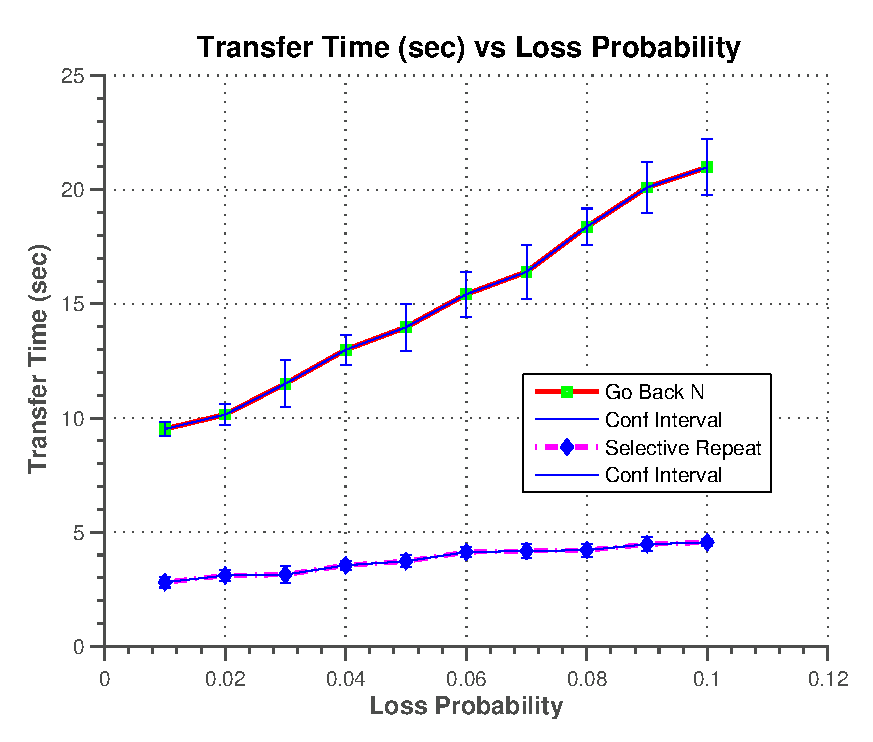
\includegraphics[width=\linewidth]{../task3/figure_task3_combined.eps}
                \caption{Average Transfer Time (sec) vs Loss Probability (p) for Go Back N and Selective Repeat Strategies.}
                \label{fig:task3combined}
        \end{subfigure}
\caption{Combined Results for Tasks 1, 2 and 3.}
\label{fig:taskscombined}
\end{figure}

The Figure \ref{fig:taskscombined} shows the combined plots for Tasks 1, 2 and 3 (Figures \ref{fig:task1combined}, \ref{fig:task2combined} and \ref{fig:task3combined} respectively) using the Go Back N and Selective Repeat Strategies for comparative purposes. These are essentially the same graphs as reported in the Sections \ref{sec:gbn}, \ref{sec:selrepeat}; the only difference being that the results for each task using both strategies are shown on the same axes.

	\printbibliography
\end{document}  